%! Author = User
%! Date = 13.09.2023

% Preamble
\documentclass[a4paper,10pt,twocolumn]{article}

% Packages 
\usepackage[utf8]{inputenc}  %man kann Sonderzeiche wie ü,ö usw direkt eingeben
\usepackage{amsmath}           %macht
\usepackage{amsfonts}          %       Mathe
\usepackage{amssymb}           %              mächtiger
\usepackage{graphicx}          %erlaubt Graphiken einzubinden (.eps für dvi und ps sowie .jpg für pdf)
\usepackage[T1]{fontenc}       %Zeichenbelegung der verwendeten Schrift
\usepackage{ae}                %macht schöneres ß
\usepackage{typearea}
\usepackage{amstex}
\usepackage{siunitx}
\usepackage{hyperref}	         %ermöglicht änderung des Seitenspiegels
\usepackage{subcaption}


\usepackage{amsmath}
\usepackage{tikz}
\usepackage{pgfplots}

\newcommand{\alphaNoError}{(4.047 \pm 0.036)}
\newcommand{\betaNoError}{(-4.73 \pm 0.29) \cdot 10^{-3}}
\newcommand{\halfTimeNoError}{(146.5 \pm 9.1)\ s}
\newcommand{\alphaGauss}{(4.04 \pm 0.10)}
\newcommand{\betaGauss}{(-4.62 \pm 0.95) \cdot 10^{-3}}
\newcommand{\halfTimeGauss}{(150 \pm 31)\ s}
\newcommand{\alphaPoisson}{(4.05 \pm 0.10)}
\newcommand{\betaPoisson}{(-4.75 \pm 0.95) \cdot 10^{-3}}
\newcommand{\halfTimePoisson}{(146 \pm 29)\ s}
\newcommand{\symN}{\delta N}



\pagestyle{scrheadings}        %sagt Koma-Skript, dass selbstdefiniers Kopfzeilen verwendet werden
\typearea{16}                  %stellt Seitenspiegel ein
\columnsep25pt								 %definiert Breite zwischen den zwei Spalten von \twocolumns

\renewcommand{\pnumfont}{%     %ändert die Schriftart der Seitennummerierung
    \normalfont\rmfamily\slshape}  %ändert die Schriftart der Seitennummerierung 



\begin{document}
    \twocolumn[{\csname @twocolumnfalse\endcsname                %erlaubt "Abstrakt" über beide Spalten
    \titlehead{                                                  %Kopfzeile
        \begin{tabular*}{\textwidth}[]{@{\extracolsep{\fill}}lr}   %Kopfzeile
            Tutor: ? & \today\\                          %Kopfzeile - Betreuer
        \end{tabular*}                                             %Kopfzeile
    }
    \title{Magnetic hysteresis curves and characteristic magnetic properties of Fe-Ni-Alloy and Steel}  %Titel der Versuchs
    \author{Salahudin Smailagić and Thomas Karb}                     %Namen der Studenten
    \date{}                                                         %benötigt um automatisches Datum auszuschalten
    \maketitle                                                      %erzeugt Titelseite
    \vspace{-5ex}                                                   %verringert Abstand zur Überschrift
    \begin{abstract}                                                %Beginn des Abstracts
        
        
        
        \\
        Measuerement made: 21. September 2023\\       %Datum ändern!
        Submitted: 26. September 2023                %Datum ändern!
        \\
        \\
    \end{abstract}
    }] 
    \section{Introduction}
    Ferromagnetic materials have a high magnetic permeability.
    In paramagnets and diamagnets the resulting magnetic field (B-Field) directly depends on the
    extern magnetic field applied (H-Field).
    In contrast in ferromagnets the resulting B-Field is also depending on the magnetisation history of the material.
    The relation of H-field and B-field is described by the hysteresis curve.
    This phenomena enables permanent magnets.
    It enables to magnetize and demagnetize materials such as iron.
    This characteristic relation described by the hysteresis is important for applications in transformers,
    electric-motors, etc.
    In this paper we examine the hysteresis curve of two specific Fe-Ni alloys and steel Sk 732.
    
    \section{Theory}
    \label{sec:Theory}
    
    The magnetic properties of a material are caused by the spins of the electrons.
    In an ferromagnetic material the individual spins of the electrons do not cancel each other out, so every atom has an
    resulting spin.
    But every spin creates a magnetic dipole moment.
    Meaning every atom carries a magnetic dipole moment.
    In a ferromagnetic material the spin of neighboring atoms couple,
    creating domains where the atomic spins are aligned. 
    Those domains also called Weiss domains are separated by small boundaries, only a few atoms wide.
    In the 'unmagnetized' state the magnetic dipole moments of each Weiss domain, cancel each other out, resulting in
    a magnetic field of zero.
    If you now apply an external magnetic field the boundaries of the Weiss domains move, so the magnetic moments of the
    domains align with the direction of the applied H-field.
    So the H-Field gets amplified by a large amount.
    
    But the Weiss domains alone, would not explain permanent magnets and hysteresis. 
    Since in an perfect isotropic cristal, if you would remove the external H-field, the boundaries of the Weiss domains
    would move back to the initial position of lowest energy. 
    Thus the material would be 'unmagnetized' again.
    
    A real material on the other hand is anisotropic.
    It has defects on the cristal lattice.
    After removing the external H-Field, the boundary walls get pinned on those defects.
    So the Weiss domains can not go back in their initial configuration, thus the material stays magnetized.
    This effect results in the hysteresis curve.
    
    You can release the walls of their pinned state by heating the material, by causing vibrations through e.g.: hammering,  
    or by applying an oscillating external B-field as shown in section ~\ref{subsec:steel}.
    
    The hysteresis curve is characterized by a multitude of properties:
    If you apply the H-field the weiss domains will align.
    Thus amplifying the B-field. 
    By increasing the H-field even more, all dipole moments will be aligned and there is no amplification anymore.
    This saturation state is characterized by the threshold $B_{sat}$.
    After wards the B-field only increases with the vacuum permeability $\mu_0$.
    Now after removing the external H-field, the remaining B-field is called remanence $B_{R}$.
    The coercivity $H_C$ is the magnetic force (H-field) the material can withstand, without being demagnetized.
    
    Moving the weiss domains, costs energy.
    This energy loss, when cycling the hysteresis curve, can be calculated with the material density $\rho$:
    
    \begin{align}
        \label{eq:EnergyLoss}
        \xi = \frac{E}{m} = \frac{1}{\rho} \oint{B dH}
    \end{align}
    
    This is the area under the hysteresis curve.
    
    \section{Experimental setup}
    
    \begin{figure}[htbp]
        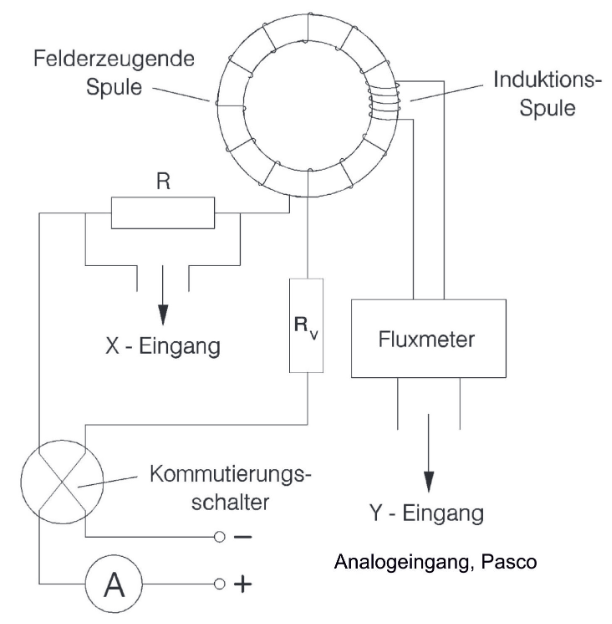
\includegraphics[width=0.9\linewidth]{ExperimentalSetup}
        \caption{Setup for capturing hysteresis curves.
        Channel X of the digital interface measures the current in the field-creating-coil $N_1$.
        The ring core conducts the H-field.
        The resulting B-field is measured by the induction-coil $N_2$.
        The flux meter integrates analog the voltage of the induction coil and its output is captured by
        channel Y.
        This enables to calculate the B-field at the induction-coil.}
        \label{fig:ExperimentalSetup}
    \end{figure}
    
    We have four ring cores of different materials.
    To capture their magnetic properties we use the experimental setup shown in figure ~\ref{fig:ExperimentalSetup}. 
    The external magnetic field is created by the first coil $N_1$.
    We measure the current via the voltage drop $U_{in}$ at the first resistor.
    Captured by the digital interface at Channel X.
    For small currents we use $R = (66.7 \pm 1.4) \Omega$, else we use $R = 0.20 \Omega$.
    The field created by the first coil can then be calculated with:
    \begin{align}
        \label{eq:CalculateHField}
        H = \frac{N_1}{\frac{\pi}{2}(d_i + d_o)R}U_{in}
    \end{align}
    Where $d_i$ and $d_o$ are the inner and outer diameter of the ring core and $N_1$ is the winding number of the
    field-creating-coil.
    
    The ring core conducts the field and induces a current in the second coil $N_2$.
    To assess the conducted B-field, we use a flux-meter, which integrates analogously, the flux change of the second coil.
    It's output is then captured by channel Y of the digital interface.
    
    The induced current depends on the effective area penetrated by the conducted field.
    \begin{align}
        \label{eq:EffectiveAreaOfInductionCoil}
        A_{eff} = \frac{1}{2} (d_o - d_i) h f
    \end{align}
    Here $h$ is the height of the second coil and $d_o$ and $d_i$ the outer and inner diameter.
    Furthermore $f$ is the effective percentage by which the ring core is filled with the ferromagnetic material.
    This has to be account for since the second and third ring core consist of $0.1 mm$ thin Fe-Ni-bands, which are coated by a oxid layer.
    The effective fill percentage of these core is $f = 90\%$.
    
    Via Ampere's law you can calculate the induced current by the B-field.
    Therefor with the integrated current measured at channel Y $U_{out}$, you can infer the conducted field:
    \begin{align}
        \label{eq:CalculateBField} 
        B = \frac{\gamma_f}{N_2 A_{eff}} U_{F}
    \end{align}
    Where $\gamma_f$ is the integration factor of the flux meter.
    
    Since the flux meter integrates analogously, there is an undetermined integration constants shifting the output
    voltage $U_{out}$.
    This shift is corrected by centering the data afterwards.
    Furthermore the flux meter has an finite input resistance, which results in a constant drift of the output voltage,
    especially for small currents.
    The following data is adjusted for both those effects.
    
    \section{Hysteresis curves}
    \subsection{Steel ST37K}
    \label{subsec:steel}
    
    \figExCoercivityRemanenceSteel{Hysteresis curve for steel ST37K\@.
    Via linear regression the coercivity $H_C = \CoercivityExCoercivityRemanenceSteel$ and remanence $B_R = \RemanenceExCoercivityRemanenceSteel$ was accessed.
    Furthermore with numerical integration the energy loss after equation~\eqref{eq:EnergyLoss} is $\xi = \HysteresisLossExCoercivityRemanenceSteel$.
    The saturation point was not reached.}
    
    We examined a ring core made of steel ST37K\@.
    The captured hysteresis curve can be seen in figure~\ref{fig:ExCoercivityRemanenceSteel}.
    To get the coercivity and remanence we apply linear regression around the H- and B-axis respectively.
    Since the the curve is in proximity of the intersection linear.
    \begin{align*}
        H_C &= \CoercivityExCoercivityRemanenceSteel \\
        B_R &= \RemanenceExCoercivityRemanenceSteel
    \end{align*}
    The error was inferred by the statistical scattering of the data points around the linear regression.
    Please be aware that this approach only reflects statistical errors.
    In our measurements we have a large amount of systematical errors, due to the fact that magnetic hysteresis is
    highly dependent on the geometry of the used ring cores. 
    To make our results reproducible, a far greater control over the geometry would be required.
    Because this paper is more concerned with qualitative results, all quantitative results only really apply for the
    local setup used by us.
    
    
    The energy loss was calculated by numerical integrating the curve and applying equation~\eqref{eq:EnergyLoss}:
    \begin{align*}
        \xi = \HysteresisLossExCoercivityRemanenceSteel
    \end{align*}
    Similarly the error was determined by the statistical scattering of the data points.
    
    \subsubsection*{Irreversibility of hysteresis}
    
    \figExIrreversibilitySteel{Hysteresis curve for ST37K.
    By briefly changing direction of the applyied H-field a hysteresis-branch is formed.
    This shows the time dependence of ferromagnetical materials. 
    It can be explained via Weiss domains (c.f. section~\ref{sec:Theory})}
    
    As stated in section~\ref{sec:Theory}, the hysteresis curve depends on the magnetization history
    of the material. 
    This effect can be revealed by briefly changing the direction of the external H-field.
    Compare figure~\ref{fig:ExIrreversibilitySteel} where after changing the field direction a branch in the curve
    is formed.
    The magnetization does not return to its previous state as would be naively expected.
    
    \subsubsection*{Demagnetization}
    
    \figExDemagnetizationSteel{}
    
    As shown in the previous section, after you reverse the polarisation of the external field, the magnetisation
    is weaker as in the previous state.
    You can use this fact to demagnetize the material.
    This was achieved by periodically flipping the H-field and decreasing its strength each step,
    The magnetic moments of the weiss domains get more and more disordered, until no remanence-field is left.
    The lowest energetic state is reached.
    
    As you can see in figure~\ref{fig:ExDemagnetizationSteel} the state of demagnetization is not
    completely reached.
    If you want to attain it perfectly, you have to flip the H-field after the coercivity is reached.
    But since we flipped the H-field manually this proved to be difficult. 
    
    \subsection{PERMENORM 5000 H2 Fe-Ni-Aloy}
    
    
    
    \subsection{PERMENORM 5000 Z Fe-Ni-Aloy}
    \subsection{Wood as reference}
    \section{Summary}
    
    
    %FF: Angabe der verwendeten Literatur mit Quellennachweis.
    \begin{thebibliography}{}    %so wird das Literaturverzeichnis erstellt
        
    \end{thebibliography}
    
\end{document}